\documentclass[../report/main.tex]{subfiles}
 
\begin{document}

\begin{enumerate}[a)]
	\item What are the lengths of the shortest paths from vertex $a$ to all other vertices?

    The shortest path problem can be solved using a linear programming model of the following form:

    maximize d_t
    subject to d_s = 0
               d_v - d_u \leq l_{u -> v} for every edge u -> v

    Based on the paths and weights denoted from the Project3Problem3-1.txt file the expressions for the linear programming solution to find shortest paths will be:

    \begin{itemize}
      \item $d_b - d_a \leq 2$
      \item $d_c - d_a \leq 3$
      \item $d_d - d_a \leq 8$
      \item $d_h - d_a \leq 9$
      \item $d_a - d_b \leq 4$
      \item $d_c - d_b \leq 5$
      \item $d_e - d_b \leq 7$
      \item $d_f - d_b \leq 4$
      \item $d_d - d_c \leq 10$
      \item $d_b - d_c \leq 5$
      \item $d_g - d_c \leq 9$
      \item $d_i - d_c \leq 11$
      \item $d_f - d_c \leq 4$
      \item $d_a - d_d \leq 8$
      \item $d_g - d_d \leq 2$
      \item $d_j - d_d \leq 5$
      \item $d_f - d_d \leq 1$
      \item $d_h - d_e \leq 5$
      \item $d_c - d_e \leq 4$
      \item $d_i - d_e \leq 10$
      \item $d_i - d_f \leq 2$
      \item $d_g - d_f \leq 2$
      \item $d_d - d_g \leq 2$
      \item $d_j - d_g \leq 8$
      \item $d_k - d_g \leq 12$
      \item $d_i - d_h \leq 5$
      \item $d_k - d_h \leq 10$
      \item $d_a - d_i \leq 20$
      \item $d_k - d_i \leq 6$
      \item $d_j - d_i \leq 2$
      \item $d_m - d_i \leq 12$
      \item $d_i - d_j \leq 2$
      \item $d_k - d_j \leq 4$
      \item $d_l - d_j \leq 5$
      \item $d_h - d_k \leq 10$
      \item $d_m - d_k \leq 10$
      \item $d_m - d_l \leq 2$
    \end{itemize}

    An image of the graph is below:

    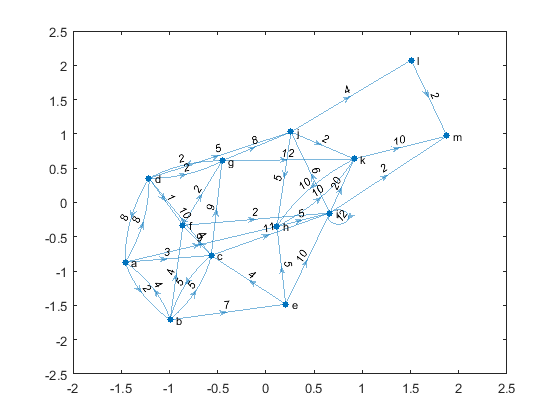
\includegraphics{../problem_three/problem3_digraph.png}

    Code used to find the shortest paths:
  
    \lstinputlisting{../problem_three/problem3_digraph_shortest_path_to_a.m}

    The lengths of the shortest paths from a to the other vertices in the graph are listed below:
    \begin{itemize}
        \item a to b: 2
        \item a to c: 3
        \item a to d: 8
        \item a to e: 9
        \item a to f: 6
        \item a to g: 8
        \item a to h: 9
        \item a to i: 8
        \item a to j: 13
        \item a to k: 15
        \item a to l: 17
        \item a to m: 10
    \end{itemize}
	\item If a vertex $z$ is added to the graph for which there is no path from vertex $a$ to vertex $z$, what will be the result when you attempt to find the lengths of shortest paths as in part a).

    Graphic with the new vertex z added:

    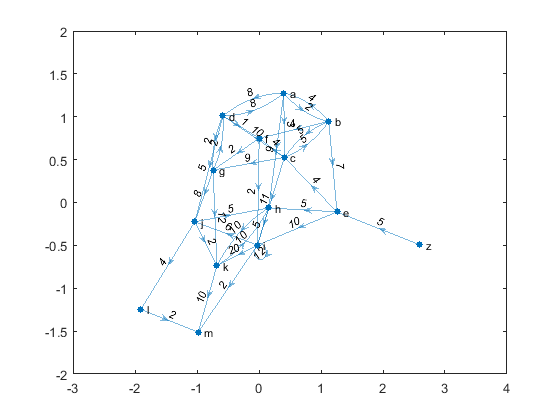
\includegraphics{../problem_three/problem3_digraph_with_z.png}

    Code used to find shortest paths from a with the new vertex z:
  
    \lstinputlisting{../problem_three/problem3_digraph_shortest_path_to_a_with_z.m}

    The list that results when the script above is executed:

    \begin{itemize}
        \item a to b: 2
        \item a to c: 3
        \item a to d: 8
        \item a to e: 9
        \item a to f: 6
        \item a to g: 8
        \item a to h: 9
        \item a to i: 8
        \item a to j: 13
        \item a to k: 15
        \item a to l: 17
        \item a to m: 10
        \item a to z: Inf
    \end{itemize}

    The list will be the same except for the addition of the line 'a to z: Inf' which shows that you cannot access vertex z from a in the current graph because that is what was specified in the question.

	\item What are the lengths of the shortest paths from each vertex to vertex $m$? How can you solve this problem with just one linear program?

    Code used to find the shortest paths from all other vertices to m:

    \lstinputlisting{../problem_three/problem3_digraph_shortest_path_to_m.m}

    \begin{itemize}
        \item a to m: 10
        \item b to m: 8
        \item c to m: 8
        \item d to m: 5
        \item e to m: 12
        \item f to m: 4
        \item g to m: 7
        \item h to m: 7
        \item i to m: 2
        \item j to m: 6
        \item k to m: 10
        \item l to m: 2
    \end{itemize}

	\item Suppose that all paths must pass through vertex $i$. How can you calculate the length of the shortest path from any vertex $x$ to vertex $y$ that pass through vertex $i$ (for all $x, y \in V$)? Calculate the lengths of these paths for the given graph. (Note: for some vertices $x$ and $y$, it may be impossible to pass through vertex $i$).
\end{enumerate}

\end{document}
